\begin{thesischapter}{1} {Marco teórico}
    En este capítulo se explican algunos de los conceptos claves utilizados en el trabajo. Además, se presenta una revisión del estado del arte y las herramientas que dan solución a algunos de los aspectos más importantes en el sistema, y se exponen
    las principales características de estas. Al final del capítulo se hace un breve resumen de la metodología de trabajo para la implementación del sistema.

    %% Conceptos teóricos
    \subthesischapter{Aspectos conceptuales en la Rehabilitación Muscular}
    
    \vspace{10pt}
    \subsubthesischapter{Accidentes Cerebrovasculares}
    Se define como accidente cerebrovascular (ACV) o Ictus a todo episodio de
    instauración súbita, aguda o subaguda, en el que, a causa de una lesión primaria o
    secundaria localizable en cualquier punto del sistema cardiovascular, se produce un
    déficit neurológico, permanente o transitorio, en relación con la zona afectada.~\cite{ictus}

    \vspace{10pt}
    \subsubthesischapter{Tipos de afecciones motoras y cognitiva}
    Los tipos y grados de discapacidad que siguen a un derrame dependen de qué área
    del cerebro esté dañada fig: \ref{fig: cerebralcortex}. Generalmente, el accidente cerebrovascular puede
    causar cinco tipos de discapacidades: parálisis o problemas para controlar el movimiento;
    trastornos sensoriales, incluyendo dolor; problemas en el uso o comprensión del
    lenguaje; problemas con el pensamiento y la memoria, y trastornos emocionales.~\cite{post-strok} 
    \begin{figure}[ht]
        \centering
        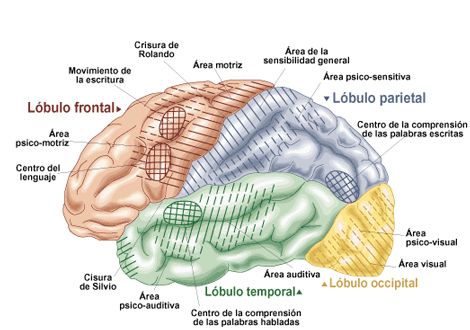
\includegraphics[scale=0.5]{images/brain.jpg}
        \caption{Áreas funcionales de la corteza cerebral}
        (Tomado de ~\cite{areacereabral})
        \label{fig: cerebralcortex}
    \end{figure}

    \begin{itemize}
        \item Parálisis o problemas para controlar el movimiento: \\
        La parálisis es una de las discapacidades más comunes causadas por un accidente
        cerebrovascular. Se suele dar en el lado del cuerpo opuesto al lado del hemisferio   dañado y
        puede afectar a la cara, un brazo, una pierna o a todo un lado del cuerpo. Esta parálisis
        unilateral se denomina hemiplejia (si la parálisis no es completa se denomina
        hemiparesia). Los pacientes con hemiparesia o hemiplejia pueden tener dificultades con
        las actividades cotidianas, como caminar o agarrar objetos.~\cite{cuidadosalpacienteadulto}
        \item Alteraciones sensoriales, incluyendo dolor:\\
        Los pacientes con accidente cerebrovascular pueden perder la capacidad de sentir
        el tacto, dolor, temperatura o posición. También pueden tener dificultad para reconocer
        objetos que están sosteniendo, e incluso pueden ser lo suficientemente graves como para
        causar la pérdida del reconocimiento de su propia extremidad. Algunos pacientes con
        apoplejía llegan a experimentan dolor, entumecimiento o sensaciones extrañas de
        hormigueo o picor en las extremidades paralizadas o debilitadas, un síntoma conocido
        como parestesias.~\cite{post-strok}
        \item Problemas para usar o comprender el lenguaje (afasia):\\
        Los sobrevivientes de accidentes cerebrovasculares experimentan deficiencias en el lenguaje, 
        que involucran la capacidad de hablar, escribir y comprender el lenguaje hablado y escrito. 
        En las personas diestras, estos accidentes cerebrovasculares generalmente involucran el lado 
        izquierdo del cerebro. Una lesión inducida por un accidente cerebrovascular en cualquiera de 
        los centros de control del lenguaje del cerebro puede afectar gravemente la comunicación verbal. 
        Hay varios tipos de afasia:~\cite{post-strok}
        \begin{itemize}
            \item Afasia expresiva, en la que las personas pierden la capacidad de hablar o escribir las palabras que están pensando y de juntar palabras en oraciones coherentes y gramaticalmente correctas.
            \item Afasia receptiva, en la que las personas tienen dificultad para comprender el lenguaje hablado o escrito y, a menudo, tienen un habla incoherente. Aunque estos individuos pueden formar oraciones gramaticalmente correctas, sus expresiones a menudo carecen de significado.
            \item Afasia global, en la que las personas pierden casi todas sus habilidades lingüísticas; no pueden entender el lenguaje o usarlo para transmitir pensamientos.  
        \end{itemize}
        \item Problemas con el pensamiento y la memoria:\\
        Un accidente cerebrovascular puede causar daño a partes del cerebro responsables
        de la memoria, el aprendizaje y la conciencia. Los pacientes pueden haber reducido
        dramáticamente su capacidad de atención o pueden experimentar déficit en la memoria a
        corto plazo. También pueden perder su capacidad de hacer planes, comprender el
        significado de las cosas, aprender nuevas tareas, o participar en otras actividades mentales
        complejas.~\cite{post-strok}
        \item Trastornos emocionales:\\
        Muchas personas tras sobrevivir a un derrame sienten miedo, ansiedad,
        frustración, ira, tristeza y un sentimiento de dolor por sus pérdidas físicas y mentales.
        Estos sentimientos son una respuesta natural al trauma psicológico del ictus. Algunos
        trastornos emocionales y cambios de personalidad son causados por los efectos físicos
        del daño cerebral.~\cite{post-strok} 
    \end{itemize}

    \vspace{10pt}
    \subsubthesischapter{Activación muscular durante el pedaleo}
    Muchos estudios de ciclismo han utilizado las señales de EMGs para comprender mejor
    cómo funcionan los músculos durante las diferentes fases del movimiento. Una de las
    particularidades observadas ocurre durante la fase de propulsión del pedaleo, donde la
    mayoría de los pares de músculos agonistas/antagonistas se activan juntos para generar
    torques durante esta fase. El análisis está basado en los tiempos de inicio y final de la
    contracción muscular y los niveles de amplitud alcanzados, sincronizados con mediciones
    cinemáticas o dinámicas del movimiento como el ángulo, la aceleración o la velocidad
    angular, torque, potencia o de marcadores de tiempo con el uso de codificadores en la
    manivela de la bicicleta o del pedal motorizado. Con ellos se ha demostrado que las
    personas sanas tienen patrones de coordinación intermusculares predecibles durante el
    pedaleo. Los cuales también están relacionados con la cadencia o revoluciones por
    minutos, la posición del cuerpo, así como con la carga de entrenamiento a la cual es
    sometido el usuario. Estos patrones suelen ser alterados en pacientes con
    discapacidades motoras debido a cambios que sufren los músculos, como el
    acortamiento ~\cite{johnston2007biomechanical}. De ahí que la señales de EMGs permiten 
    detectar los grupos musculares dañados y enfocar el entrenamiento hacia estos 
    ~\cite{hug2009electromyographic, kautz1998relationships}

    \vspace{10pt}
    Según~\cite{Losmúscu21}, los grupos musculares que intervienen en el pedaleo son:

    \begin{itemize}
        \item \textbf{Los cuádriceps} son un grupo de cuatro músculos situados en la parte frontal del muslo. Estos músculos incluyen el recto femoral(RF), el vasto lateral(VL), el vasto intermedio(VI) y el vasto medial(VM). Durante el pedaleo, los cuádriceps se contraen para extender la pierna en la rodilla durante la fase de empuje hacia abajo del pedal. Esta acción proporciona la potencia necesaria para superar la resistencia y avanzar con eficiencia.
        
        \item Situados en la parte posterior del muslo, \textbf{los isquiotibiales} son otro grupo muscular clave en el pedaleo. El bíceps femoral(BF), el semitendinoso(ST) y el semimembranoso(SM) son los músculos principales de esta zona. Durante la fase de levantamiento del pedal, los isquiotibiales se activan para flexionar la pierna en la rodilla y extender la cadera. Este movimiento se encarga de levantar el pedal y preparar la siguiente fase de empuje.
        
        \item \textbf{Los gemelos}(GM, GL) y \textbf{el sóleo}(SOL) se encuentran en la pantorrilla y también participan en el pedaleo. Son cruciales para la flexión plantar del pie durante la fase de empuje hacia abajo del pedal. Su acción ayuda a generar potencia y proporciona estabilidad en el tobillo durante el pedaleo.
        
        \item Localizados en la parte frontal de la espinilla, \textbf{los tibilales anteriores}(TA) intervienen en la flexión dorsal del pie durante la fase de levantamiento del pedal. Esta acción es esencial para mantener el equilibrio y preparar la pierna para el siguiente empuje.
        
        \item Aunque su papel es menos evidente, los \textbf{glúteos}(G) también son importantes en el pedaleo. Tanto el glúteo mayor como el glúteo medio contribuyen a la extensión de la cadera y ayudan a potenciar el movimiento durante la fase de empuje del pedal.
    \end{itemize}

    \vspace{10pt}
    La figura~\ref{fig: musculegroups} muestra detalles gráficos de los grupos musculares mencionados.

    \begin{figure}[ht]
        \centering
        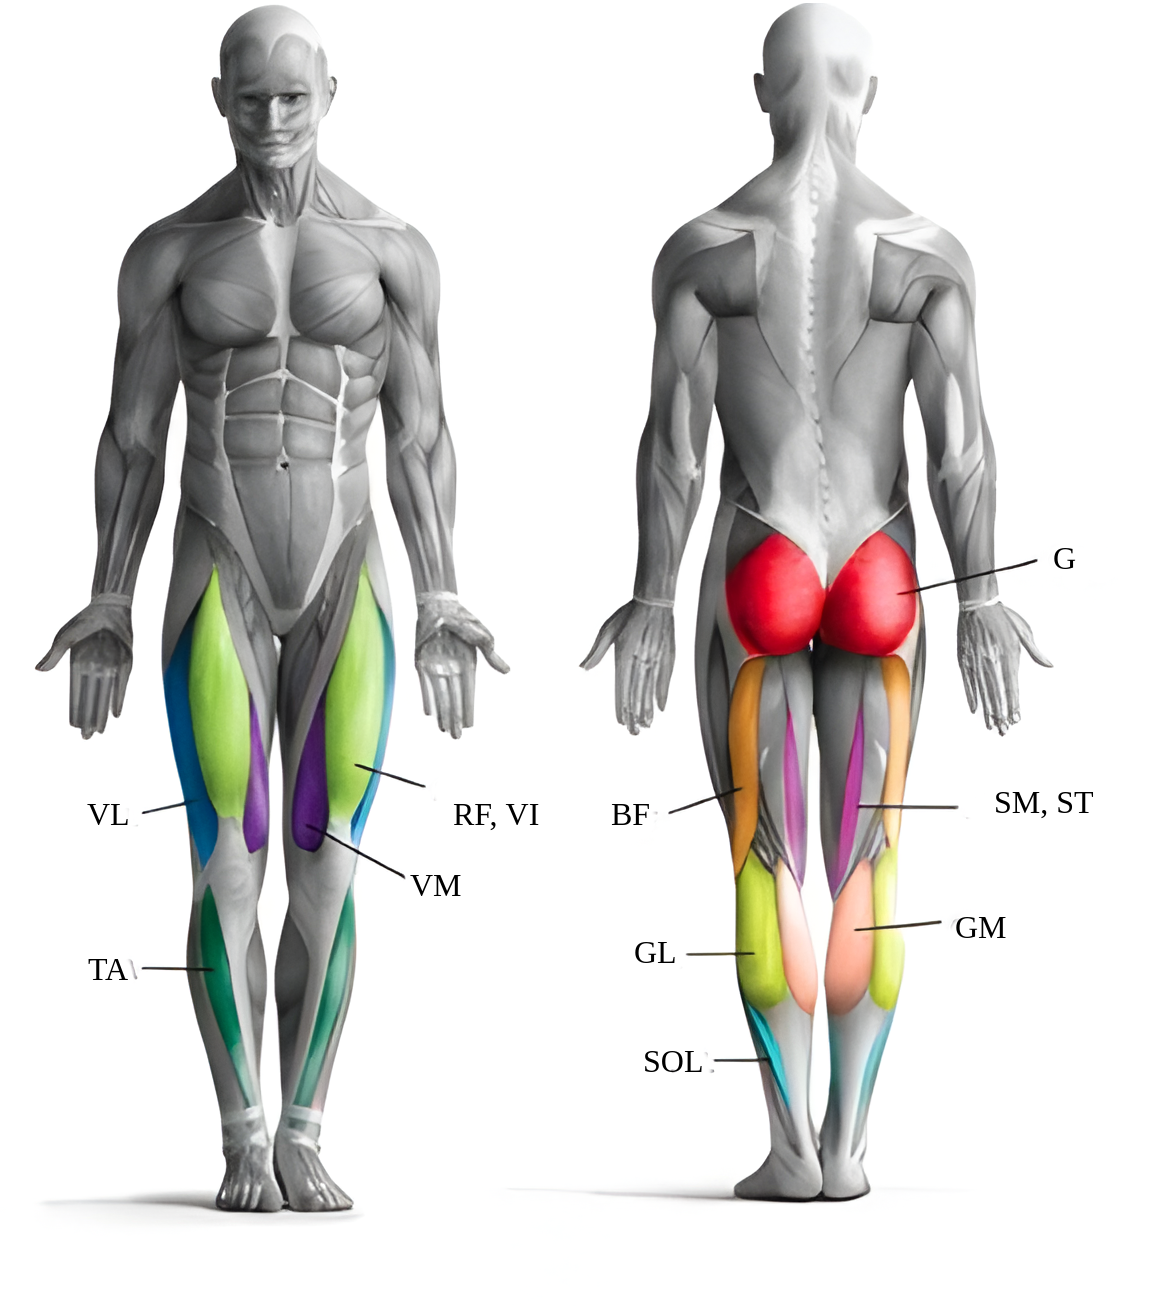
\includegraphics[scale=0.2]{images/musculegroups.png}
        \caption{Grupos musculares usados en pedaleo}
        (Tomado de ~\cite{Quémúsc72})
        \label{fig: musculegroups}
    \end{figure}

    \vspace{10pt}
    \subsubthesischapter{Tecnologías de la Rehabilitación}
    Las denominadas tecnologías en rehabilitación se puede concebir como el conjunto de productos y conocimientos
    desarrollados desde avances tanto en la ingeniería de la rehabilitación como en las profesiones y disciplinas 
    que estudian el fenómeno de la discapacidad. En este orden de ideas, la tecnología en rehabilitación estudia 
    no sólo lo relacionado con el desarrollo y la producción de instrumentos, equipos, sistemas o dispositivos, 
    que contribuyan a procesos de rehabilitación, sino que se interesa, además, por el impacto de estos elementos en el desempeño y la capacidad funcional de las personas con discapacidad, en el acceso
    de estas personas y sus familias a los adelantos tecnológicos y en el nivel de uso que se les da,
    además de lo relacionado con la accesibilidad y diseño.\cite{matheus1990tecnologia}

    \vspace{10pt}
    Un término que regularmente se utiliza en este campo es el de tecnología de asistencia, que
    no debe equipararse al de ingeniería de la rehabilitación ni al de tecnología de la rehabilitación, ortesis o 
    prótesis, pues no son idénticos. En esta perspectiva Bronzino y Cols.~\cite{enderle2012introduction}  mencionan que:

    \begin{itemize}
        \item  La tecnología de asistencia es la utilización de cualquier parte de un equipo o sistema productivo modificado o comercializado, para incrementar o mejorar capacidades funcionales de un individuo. Esta definición ve
        la tecnología de asistencia como una serie de aparatos, estrategias y/o servicios, que ayudan al individuo a realizar mejor una actividad; en consecuencia, incluye desde baja
        tecnología, que es poco costosa, hasta alta tecnología, que es costosa y con productos de compleja fabricación. Como ejemplos de baja
        tecnología se incluyen utensilios de doble agarre, cepillos para la boca, entre otros; y de
        alta tecnología aparatos de comunicación computarizada, máquinas lectoras con inteligencia artificial y brazos artificiales
    \end{itemize}
    
    \vspace{10pt}
    \textbf{Modalidades de Rehabilitación} \\ 
    La terapia con dispositivos róboticos de pedaleo se clasifica, al igual que las terapias
    convencionales, en modo pasivo, activo y activo asistido \cite{barclay2019effect}. Estos diferentes enfoques
    se preescriben según el grado de las secuelas que padece el paciente, el nivel de
    conciencia de este y las diferentes fases del proceso de rehabilitación en que se
    encuentran. El ciclismo con estos fines consiste que los usuarios ejecuten movimientos
    circulares, similares a los realizados en una bicicleta.

    \vspace{5pt}
    En el ciclismo activo, la persona al pisar o agarrar el pedal es capaz de continuar el
    ejercicio por sí solo. Durante esta modalidad, el paciente debe ir venciendo gradualmente
    las resistencias opuestas al movimiento. De esta manera el tratamiento es denominado
    como resistido y su objetivo principal es el fortalecimiento de los músculos involucrados.
    En el modo pasivo, los miembros afectados siguen la trayectoria y velocidad programada
    para los pedales \cite{ferreira2020virtual}. Este modo es también empleado en la rehabilitación activa asistida,
    la cual es aplicada a los pacientes que debido a la disminución de la fuerza muscular,
    inician el movimiento activo pero no son capaces de recorrer todo el arco articular \cite{cruz2009guia}.
    En este caso las tecnologías de pedaleo permiten la transición de forma automática o
    manual del entrenamiento activo al pasivo y viceversa.

    \vspace{5pt}
    El ciclismo pasivo es adecuado al principio de la rehabilitación, pues contribuye a la
    regulación del tono muscular, relajación de la musculatura y prevención de las dificultades
    que trae consigo estar inactivo o inmovilizado, disminuyendo así las probabilidades de
    complicaciones a largo plazo \cite{cruz2009guia}. El inicio temprano de intervenciones de ejercicios de
    pedaleo desde la cama en pacientes críticamente enfermos puede ayudar a reducir la
    sarcopenia y recuperar la fuerza muscular \cite{nickels2020acceptability}. También es indicado para reducir la
    inflamación, aliviar el dolor y recuperar el rango de movimiento. Además, se ha
    comprobado un mejoramiento en el sistema cardiovascular y respiratorio después de la
    terapia pasiva \cite{cruz2009guia, phadke2019impact}.
    Esta modalidad es particularmente útil en pacientes con déficit severo que no tienen
    control o potencia motriz suficiente para participar en movimientos activos, por ejemplo,
    sujetos con LM completa \cite{phadke2019impact, nardone2017passive}. Phadke et al \cite{phadke2019impact} reflejaron en una revisión sistemática
    notables efectos del ciclismo pasivo en miembros inferiores para personas con esta
    condición. En las intervenciones clínicas analizadas por estos autores, los efectos
    positivos fueron más evidentes tras la realización de múltiples sesiones. Entre los efectos
    cardiovasculares, se observó un incremento del flujo sanguíneo en las piernas con la
    consecuente disminución de la resistencia vascular periférica. En el sistema
    músculoesquelético, hubo un mantenimiento e incremento del RDM de las articulaciones
    y una atenuación de la atrofia muscular. Además, fue comprobada la influencia de los
    ejercicios pasivos en el SNC, donde los indicadores mostraron una disminución
    significativa de la espasticidad (evaluada tras la medición de la amplitud del reflejo H) y
    de la inhibición intracortical. En los pacientes con EM, el ciclismo pasivo también ha
    producido estos efectos antiespásticos \cite{motl2006effect, guyot2012effects}. Todas estas repercusiones generalmente
    son apreciadas a partir de la realización de pedaleo activo \cite{nardone2016effects}, sobre todo en sujetos
    sanos, de ahí la importancia de conocer que el pedaleo pasivo también produzca efectos
    similares.

    \vspace{5pt}
    El ciclismo activo-asistido ha producido mejoras en la función motora de los pacientes
    con EP, particularmente el temblor y la bradicinesia \cite{ryan2020interval, palomino2021efectividad}. 
    Esta modalidad es
    aprovechada para su uso con terapias complementarias como la estimulación eléctrica
    funcional (EEF). Esta técnica ha sido considerada desde hace varios años como un
    método bien establecido y estandarizada en la rehabilitación de pacientes con
    enfermedades neurológicas como las ACV \cite{rabelo2018overview}. El ciclismo asistido por EEF es un
    enfoque utilizado con fines de re-habilitación que contribuye a restaurar el trofismo
    muscular y aumentar la fuerza muscular \cite{barbosa2015application, ferrante2008cycling}. El principio de funcionamento se basa
    en estimular las unidades motoras para activar los músculos paralizados o paréticos
    durante la realización de tareas funcionales. Diferentes estudios han evaluado la eficacia
    de la EEF combinada con el ciclismo en la recuperación motora, principalmente en
    pacientes con ACV \cite{ambrosini2020does}, LM \cite{casabona2020effects} y EM \cite{pilutti2019functional}. También se ha evidenciado beneficios
    positivos sobre la capacidad aeróbica máxima, el control postural, la espasticidad y la
    coordinación motora \cite{barbosa2015application, rabelo2018overview}.
    


    \subthesischapter{Aspectos conceptuales en sistemas informáticos.}
    \vspace{10pt}
    \subsubthesischapter{Arquitectura Cliente-Servidor}
    Según ~\cite{moyano2020arquitectura} la arquitectura Cliente - Servidor, es 
    un modelo de una aplicación distribuida en el cual se basa en dos actores:
    Uno con rol de proveedor de recursos y otro con rol consultor sobre los recursos.
    \begin{itemize}
        \item Cliente: Programa ejecutable que participa activamente en el establecimiento de las conexiones. Envía una petición al servidor y se queda
        esperando por una respuesta. Su tiempo de vida es finito una vez que son
        servidas sus solicitudes, termina el trabajo.
        \item Servidor: Es un programa que ofrece un servicio que se puede obtener
        en una red. Acepta la petición desde la red, realiza el servicio y devuelve
        el resultado al solicitante. Al ser posible implantarlo como aplicaciones de
        programas, puede ejecutarse en cualquier sistema donde exista TCP/IP y
        junto con otros programas de aplicación. El servidor comienza su ejecución
        antes de comenzar la interacción con el cliente.
    \end{itemize}

    \vspace{10pt}
    \subsubthesischapter{Motores Gráficos}

    \vspace{2pt}
    Un motor de videojuegos es una aplicación de software que ofrece todas las herramientas necesarias para el diseño y desarrollo completo de un videojuego, disponiendo de un motor de renderizado para gráficos 2D y 3D, detector de colisiones, sonidos, scripting, animación, inteligencia artificial, redes, streaming, administración de memoria y mucho más \cite{arce2011desarrollo}.
    
    \vspace{10pt}
    \subsubthesischapter{Protocolos de Comunicación TCP/IP}
    TCP/IP es un conjunto de protocolos que especifican estándares de comunicaciones entre sistemas y detallan los convenios para el direccionamiento y la interconexión de redes. El protocolo TCP/IP permite las comunicaciones entre varios sistemas (llamados sistemas principales) conectados en una red. A su vez, cada red puede estar conectada a otra para comunicarse con los sistemas principales de dicha red. Aunque existen muchos tipos de tecnologías de red, algunas de las cuales utilizan el transporte en modalidad continua y por conmutación de paquetes, TCP/IP ofrece una ventaja importante: la independencia de hardware ~\cite{protocolo-tcp-ip}.

    \vspace{10pt}
    \subsubthesischapter{Base de Datos}
    Una base de datos es una recopilación organizada de información o datos estructurados, que normalmente se almacena de forma electrónica en un sistema informático. Normalmente, una base de datos está controlada por un sistema de gestión de bases de  datos (SGBD). En conjunto, los datos y el DBMS, junto con las aplicaciones asociadas a ellos, reciben el nombre de sistema de bases de datos, abreviado normalmente a simplemente base de datos.~\cite{Quéesuna68}

    \vspace{10pt}
    \textbf{Sistemas de gestión de Bases de Datos} \\
    Normalmente, una base de datos requiere un programa de software de bases de datos completo, conocido como sistema de gestión de  bases de datos (SGBD). Un SGBD sirve como interfaz entre la base de datos y sus programas o usuarios finales, lo que permite a los  usuarios recuperar, actualizar y gestionar cómo se organiza y se optimiza la información. Un SGBD también facilita la supervisión y el control de las bases de datos, lo que permite una variedad de operaciones administrativas como la supervisión del rendimiento, el ajuste, la copia de seguridad y la recuperación.~\cite{Quéesuna68}

    \vspace{10pt}
    Entre los SGBD relacionales más modernos se encuentran [33]:
    \begin{itemize}
        \item MySQL: Es un sistema relacional de código abierto, multihilo y multiusuario. Código
        abierto significa que todo el mundo puede acceder a1 código fuente, es decir, a1 código de
        programación del SGBD, en este caso MySQL ~\cite{ian2003biblia}. Presenta como ventajas principales: alta
        velocidad al realizar las operaciones, bajo costo en requerimientos para la elaboración de
        bases de dato, facilidad de configuración, instalación, usabilidad y administración. MySQL
        puede ejecutarse en la inmensa mayoría de sistemas operativos y tiene compatibilidad en su
        mayor parte con los lenguajes de programación ANSI C y C++.
        \item Microsoft SQL Server: Es un sistema basado en el lenguaje Transact-SQL, capaz de poner
        a disposición de muchos usuarios grandes cantidades de datos de manera simultánea. Es un
        sistema propietario de Microsoft. Sus principales características son: soporte de
        transacciones, alta escalabilidad, estabilidad y seguridad. Incluye también un potente entorno
        gráfico de administración. Su principal desventaja es el precio, aunque cuenta con una
        versión EXPRESS que permite usarlo en entornos pequeños.
        \item Oracle: Es un sistema multiplataforma fabricado por Oracle Corporation. Tradicionalmente
        ha sido el SGBD por excelencia, considerado como el más completo y robusto; destacado
        por su soporte de transacciones, alta estabilidad y escalabilidad. También siempre ha sido
        considerado de los más caros, por lo que no se ha estandarizado su uso como otras
        aplicaciones. Al igual que SQL Server, Oracle cuenta con una versión EXPRESS gratis para
        pequeñas instalaciones o usuarios personales.
        \item Microsoft Access: Es un sistema creado por Microsoft para uso personal de pequeñas
        organizaciones. Una posibilidad adicional es la de crear ficheros con bases de datos que
        pueden ser consultados por otros programas. Este SGBD permite crear tablas de datos
        indexadas, modificar tablas de datos, creación de consultas, formularios, informes, vistas de
        diseño y consultas referencias cruzadas.
        \item PostgreSQL: Es uno de los líderes de los sistemas de gestión de base de datos (SGBD)
        relacionales de código abierto. Este gestor de BD es uno de los almacenes de datos más rápido
        y potente del mercado debido a sus características avanzadas (extensibilidad, seguridad y
        estabilidad). Dado a que no tiene restricción en su entrada a datos, usa multiprocesos en vez
        de multihilos para garantizar la seguridad del sistema, un fallo en uno de los procesos no
        afectará el resto y el sistema continuará funcionando. Ofrece, al igual que MySQL, un sistema
        de contraseñas y privilegios seguros mediante verificación basada en el host, y el tráfico de
        contraseñas está cifrado al conectarse a un servidor. Además, este gestor de BD soporta gran
        cantidad y variedad de datos y tiene compatibilidad en su mayor parte con los lenguajes de
        programación Java, C y C++, entre otros
        \item SQLite: Es una biblioteca utilizada en multitud de aplicaciones actuales ya que es open 
        source y las consultas son muy eficientes. Las principales características de SQLite son:
        \begin{itemize}
            \item El tamaño, al tratarse de una biblioteca, es mucho menor que cualquier SGBD
            \item Reúne los cuatro criterios ACID (Atomicidad, Consistencia, Aislamiento y Durabilidad) logrando gran estabilidad
            \item Gran portabilidad y rendimiento
        \end{itemize}
    \end{itemize}

    \vspace{10pt}
    \subthesischapter{Juegos Serios}
    Los videojuegos interactivos han surgido como nuevos enfoques de tratamiento en la rehabilitación del accidente cerebrovascular. Estos enfoques pueden ser ventajosos ya que dan la oportunidad de practicar actividades que no se pueden realizar dentro del entorno clínico. Además, los programas de realidad virtual están diseñados para ser más interesantes y agradables que las terapias tradicionales, alentando que el paciente realice un mayor número de repeticiones de los ejercicios~\cite{laver2018virtual,alfageme2002aprendiendo}

    \vspace{10pt}
    En el área de la rehabilitación %dirigida a pacientes con afecciones cerebrovasculares 
    existen diferentes contribuciones dirigidas a la recuperación y rehabilitación de las diferentes habilidades y competencias psicomotrices. 
    A continuación se presentan las propuestas más relevantes que existen actualmente usando juegos serio:
    \begin{itemize}
        \item En el 2019, ~\cite{rodriguez2019design} presentó un juego serio para propósitos de rehabilitación a personas con ACV. El juego utiliza el software de desarrollo para entornos Unity 3D en su versión libre. El sensor que realiza el seguimiento de los movimientos de la persona es el sensor Kinect. El objetivo del juego consiste en que el usuario agarre esferas de un color específico. Los puntajes alcanzados en el juego y los parámetros de configuración colocados por el kinesiólogo son almacenados junto con la información del paciente. De esta manera el fisioterapeuta puede recuperar los datos almacenados y realizar un análisis de la evaluación de la evolución de la persona en su rehabilitación. 
        \item Alberto y Edwin Daniel ~\cite{morales2019desarrollo} proponen una aplicación de juego serio para tratar de aumentar y de evaluar el límite de estabilidad de la población envejecida. Tras esta idea, se hacen uso del sensor Kinect V1 y el motor de juego Unity3D, compatible mediante el uso de la librería \textit{Kinect with MS-SDK}, para poder registrar los movimientos del paciente durante la terapia. El juego basará su fundamento clínico en diversos test de evaluación del balance, como son el test Fugl-Meyer o el Choice Stepping Reaction Time, y tomará como mecánica de referencia la de uno de los clásicos de los videojuegos, el Tetris. Blocks Rehab, la adaptación clínica de este juego de los años 80, consistirá en tres modalidades de juego (Bloques, Puzzle y E.T. Tris), cumpliendo cada uno de ellos una función específica. El paciente deberá desplazarse de manera frontal, lateral y mantener el equilibrio sobre una pierna para llevar a cabo los objetivos que el videojuego les plantea, con el propósito de extraer métricas de salida que evalúen la actuación del usuario en términos de estabilidad. 
        \item En la revisión realizada por ~\cite{doi:10.1177/1545968314535985}, se comparó el efecto de realizar el entrenamiento con un soporte de brazo, combinado con ejercicios mediante un juego de realidad virtual y la rehabilitación convencional en pacientes con ictus.\\ El dispositivo que utiliza el soporte para el brazo se llama ArmeoBoom. Está compuesto de un sistema de suspensión en cabestrillo elevado, que proporciona un soporte para la muñeca. Este elemento proporciona un buen soporte en un espacio tridimensional que te permite realizar movimientos funcionales sin ninguna restricción. El mecanismo se adapta a la situación física de cada paciente. ArmeoBoom está compuesto por una webcam y un ordenador portátil que permiten al usuario interaccionar con los videojuegos incorporados en el ordenador portátil y jugar moviendo la extremidad afectada en un ambiente tridimensional ajustado al grado de movimiento funcional de cada paciente. Los movimientos, tanto en el plano horizontal como el plano vertical son controlados y grabados con la finalidad de premiar con puntos dependiendo de la actuación del usuario y del tiempo de ejecución.
        
        \vspace{2pt}
        Entrenar con el soporte de brazo consiste en realizar los movimientos con el brazo afectado, con el objetivo de maximizar la habilidad de los ejercicios usando el mínimo soporte de brazo posible.
        
        \vspace{2pt}
        El entrenamiento de rehabilitación convencional consiste en la realización de unos ejercicios ejecutados con los brazos, dirigidos por el terapeuta, para reflejar la terapia física y ocupacional. El objetivo de este entrenamiento es que el paciente incremente el rango de movimiento del brazo, principalmente del hombro y el codo con el mínimo soporte posible de una superficie como una mesa. Todos los ejercicios son análogos en esencia y consisten en alcanzar objetos colocados en una mesa, en mover o apilar vasos, colocar discos o transportar bloques de pinzas sin la ayuda de ningún ordenador ni soporte informático. Conforme el paciente va superando los juegos propuestos, los movimientos se van complicando un poco más.

        \vspace{2pt}
        Un total de 70 pacientes que habían padecido un ictus hemorrágico o isquémico en las últimas 12 semanas y que estaban estables con su medicación fueron elegidos para la rehabilitación. Los participantes pasaron por un programa de entrenamiento de seis semanas, divididas en tres sesiones de 30 minutos cada una.
        
        \vspace{2pt}
        Un grupo de 35 pacientes se formó para la rehabilitación de las extremidades superiores en combinación con el soporte de brazo y el ejercicio, mientras que 33 pacientes realizaron la rehabilitación con los ejercicios convencionales.
        
        \item En el 2014  autores como ~\cite{10.3233/NRE-141105}, comparan el efecto que se produce al entrenar con un videojuego de realidad virtual Kinect Xbox 360 Paddle Panic Mini Game, en pacientes que han padecido un ictus. El objetivo es mejorar el movimiento de la extremidad superior, observando el hemisferio cerebral afectado de estos pacientes.

        La evaluación se lleva a cabo mediante la acción de beber un vaso de agua antes y después de entrenar. Se seleccionaron un total de 40 participantes para realizar el estudio. El grupo inicial se subdividió en cuatro grupos atendiendo a los siguientes criterios:

        \begin{itemize}
            \item Pacientes con afectación derecha del cerebro (hemiparesia izquierda)
            \item Pacientes con afectación izquierda del cerebro (hemiparesia derecha)
            \item Pacientes sanos que entrenaron con la extremidad superior derecha en el videojuego
            \item Pacientes sanos que entrenaron con la extremidad superior izquierda en el videojuego
        \end{itemize}

        Los resultados del estudio muestran que los pacientes con la afectación de la  superior por ictus presentaron una mejoría del entrenamiento con el videojuego, demostrado un incremento de la puntuación en cada jugada.
    \end{itemize}

    \vspace{5pt}
    Las terapias con juegos serios son una alternativa complementaria a las terapias tradicionales. Tanto los estudios que se apoyan en tecnologías de realidad virtual, como Kinect y Nintendo, las cuales no tienen propósitos clínicos, como los que se centran en juegos serios diseñados específicamente para la rehabilitación física de diferentes patologías, indican que estos juegos tienen el potencial de mejorar el equilibrio, el control postural y
    la condición física de los pacientes, sin embargo los estudios son pocos y demasiado pequeños para llegar a una conclusión completamente fiable. La falta de eventos adversos reportados (como mareos, dolor de cabeza o náuseas) sugiere que este enfoque de la terapia es relativamente seguro, aunque esto puede variar dependiendo de las características de la persona, el hardware y el software de la realidad virtual y la tarea. 

    %%-----------------------------------------------------------
    \subthesischapter{Tecnologías y herramientas}
    \subsubthesischapter{Motor gráfico(Unity3D)}
    Actualmente podemos encontrar una amplia gama de motores de videojuegos, con diferentes tipos de licencias y orientados a cumplir distintos tipos de propósitos. Se puede encontrar motores comerciales y gratuitos, con metodologías 2D o 3D, inclusive que brindan soluciones de juegos a variadas plataformas (Windows, Linux, Android, etc.).\\ 
    
    % Afortunadamente existe una nueva tendencia por parte de algunas empresas que desarrollan motores de 
    % videojuegos, que los impulsa a colocar en el mercado versiones gratuitas (generalmente limitadas en 
    % algún aspecto) de sus herramientas para que las personas que deseen aprender, puedan hacerlo sin tener 
    % que comprar una versión full. Entre estas empresas podemos encontrar las conocidas Epic Games
    % y Unity Technologies, las cuales ofrecen versiones gratuitas y descargables de sus famosos motores de videojuegos \cite{arce2011desarrollo}.
    
    \vspace{10pt}
    La tabla 1 muestra detalles comparativos de los motores gráficos más usados del mercado:
    \begin{table}[ht]
        \centering
        \begin{tabularx}{\textwidth}{|X|X|X|X|X|X|X|}
            \hline
            \textbf{Motor gráfico  \& Atributos} & \textbf{Unity} & \textbf{Unreal Engine} & \textbf{GameMaker Studio} & \textbf{Godot} & \textbf{CryEngine}\\\hline
            Orientación                 & 2D y 3D                                                       &2D y 3D                                                          & 2D                            & 2D y 3D               & 3D \\\hline
            Sistema Operativo           & Windows, Linux, MacOS                                           & Windows                                                         & Windows                       & Windows, Linux, MacOS               & Windows, Linux, MacOS\\\hline
            Plataformas                 & iOS, Android, Window, PS4, MacOS,  Linux, Xbox One y 360, HTML5 & iOS, Android, Window, PS4, MacOS,  Linux, Xbox One y 360, HTML5   & Windows, MacOS, Linux, HTML5, Android, iOS, Amazon Fire TV, Android TV, Universal Windows Platform, PlayStation 4, Xbox One, Nintendo Switch    & Windows, MacOS, Linux    & Windows, Linux, Nintendo Switch, Xbox One, PlayStation 4, Xbox 360, PlayStation 3, Wii U\\\hline
            Lenguaje de Programación    & C\#                                                           & C++                                                             & Lenguaje propio GML           & Lenguaje de scripting & Programación basada en nodos \\\hline
            Licencia                    & Gratuita                                                      & De pago                                                         & Versión gratuita limitada     & Gratuita              &  Gratuita en la versión 5\\\hline
            Documentación               & Muy amplia                                                    & Escasa                                                          & Amplia                        & limitada              & Amplia\\\hline
            Curva de aprendizaje        & Sencilla                                                      & Complicada                                                      & Media                         & Media                 & Media \\\hline
            
        \end{tabularx}
        \label{tab: graphics-engines}
        \caption{ Tabla comparativa de los motores gráficos \\ (Adaptado de~\cite{gonjar2019desarrollo})}
    \end{table}
    
    
    \vspace{10pt}
    % Según lo antes expuesto podemos concluir en que cada uno de los motores poseen características únicas que los diferencian entre sí a 
    % la hora del desarrollo de videojuego tanto en 2d, 3d o RV.
    Para el propósito de la tesis se considera Unity como unos de los motores más populares a la hora del desarrollo de videojuegos, para las distintas plataformas, una gran ventaja que tiene Unity a la hora de desarrollar un videojuego para Android, es su modo de configurar el entorno, porque solo se necesita descargar los módulos de Android, y ya está listo para crear juegos.

    \vspace{5pt}
    Principales características de este motor gráfico que son de utilidad en el sistema:~\cite{unity3d}

    \begin{itemize}
        \item Programación con C\#.
        \item Soporte parcial de .NET (incluye soporte a .NET Sockets).
        \item Soporte de plugins para código nativo.
        \item Incluye el motor físico PhysX de Nvidia.
        \item Carga de modelados y texturas de varios formatos de programas externos como Blender, Maya, Adobe Suite, 3D Max, Cinema 4D, entre otros.
        \item Despliegue gratis sobre Android.
        \item Inspector para clases personalizadas en tiempo de ejecución.
        \item Animación a través de cinemática directa e inversa.
    \end{itemize}

    \subsubthesischapter{Visual Studio Code}
    Visual Studio Code es un editor de código fuente desarrollado por Microsoft para Windows, Linux, macOS y Web. Incluye soporte para la depuración, control integrado de Git, resaltado de sintaxis, finalización inteligente de código, fragmentos y refactorización de código, características que lo convierten en una herramienta perfecta para manipular los scripts en Unity \cite{vscode}.

    \subsubthesischapter{NET Framework 4.7}
    El framework .NET provee un modelo de programación global que permite el desarrollo de todo tipo de aplicaciones desde móviles a web a escritorio. Técnicamente el framework .NET es un ambiente de ejecución que administra las aplicaciones que corren sobre este. En él se brinda un conjunto extensivo de bibliotecas para dar solución a las principales áreas del desarrollo de software.

    El framework en sí consiste de dos grandes componentes: motor de ejecución CLR (Common Language Runtime, por sus siglas en inglés) el cual se encarga de la ejecución de las aplicaciones; y la biblioteca de clases (nombre en inglés .NET Framework Class Library)~\cite{netframework}

    \vspace{2pt}
    Características principales:
    \begin{itemize}
        \item Manejo de memoria automático.
        \item Sistema común de tipado. O sea, los tipos de datos primitivos son definidos por el framework, lo cual facilita las operaciones entre distintos lenguajes que usan este ambiente de ejecución.
        \item Una biblioteca bien vasta para operaciones generales de bajo nivel.
        \item Operatividad entre lenguajes. O sea, se puede acceder a rutinas y bibliotecas (dinámicas y estáticas) escritas en otros lenguajes si fueron compiladas con compiladores para esos lenguajes que soporten el framework .NET.
        \item Gran número de lenguajes disponibles: Visual Basic, C\#, Visual F\#, C++, entre otros.
        \item Es posible crear compilados que funcionen en múltiples plataformas de la .NET.
    \end{itemize}

    \subthesischapter{Metodología de trabajo}
    Existen diferentes modelos y metodologías que han sido utilizados en los últimos años como herramientas de apoyo para el desarrollo del software. La interrogante principal está en conocer cuál modelo utilizar en el proceso de desarrollo de software en un proyecto \cite{DELGADOOLIVERA2021}.
    
    \vspace{2pt}
    Para el desarrollo de nuestra aplicación se hará uso del modelo RAD que permite la construcción de software basada en módulos, utilizando herramientas de software que permitan de forma ágil y efectiva realizar una aplicación con altos estándares de calidad en un corto período de tiempo. Esto se debe a que un sistema completamente integrado e interdependiente entre cada una de sus partes era muy difícil de adaptar a los distintos cambios de requisitos. Además, el diseño modular del mismo brinda la posibilidad de migrar el sistema a otras tecnologías distintas o más modernas, con relativa facilidad.
    
    \vspace{2pt}
    El sistema se desarrollará de manera iterativa, donde en cada iteración se realizará un acercamiento a una versión más definitiva de un componente o módulo en específico. De esta forma siempre habrá una sección del producto parcialmente terminada que podía ser mostrada, para adaptarla a las sugerencias y peticiones de los usuarios.

    \subthesischapter{Conclusiones del capítulo}
    En este capítulo se abordó conceptos importantes para la comprensión de las soluciones e implementaciones de los distintos módulos del sistema. Se presentó el estado del arte de los juegos serios asociados a las tecnologías de rehabilitación. Adicionalmente se expusieron las principales características de las tecnologías y herramientas seleccionadas para la implementación del sistema. Finalmente se abordó la metodología de trabajo usada para desarrollar el sistema. 
\end{thesischapter}